\usetikzlibrary{matrix}
\begin{frame}{autoconfiguration}
    \begin{itemize}
    \item how do hosts get address + default routing table?
    \item one answer: set manually
    \end{itemize}
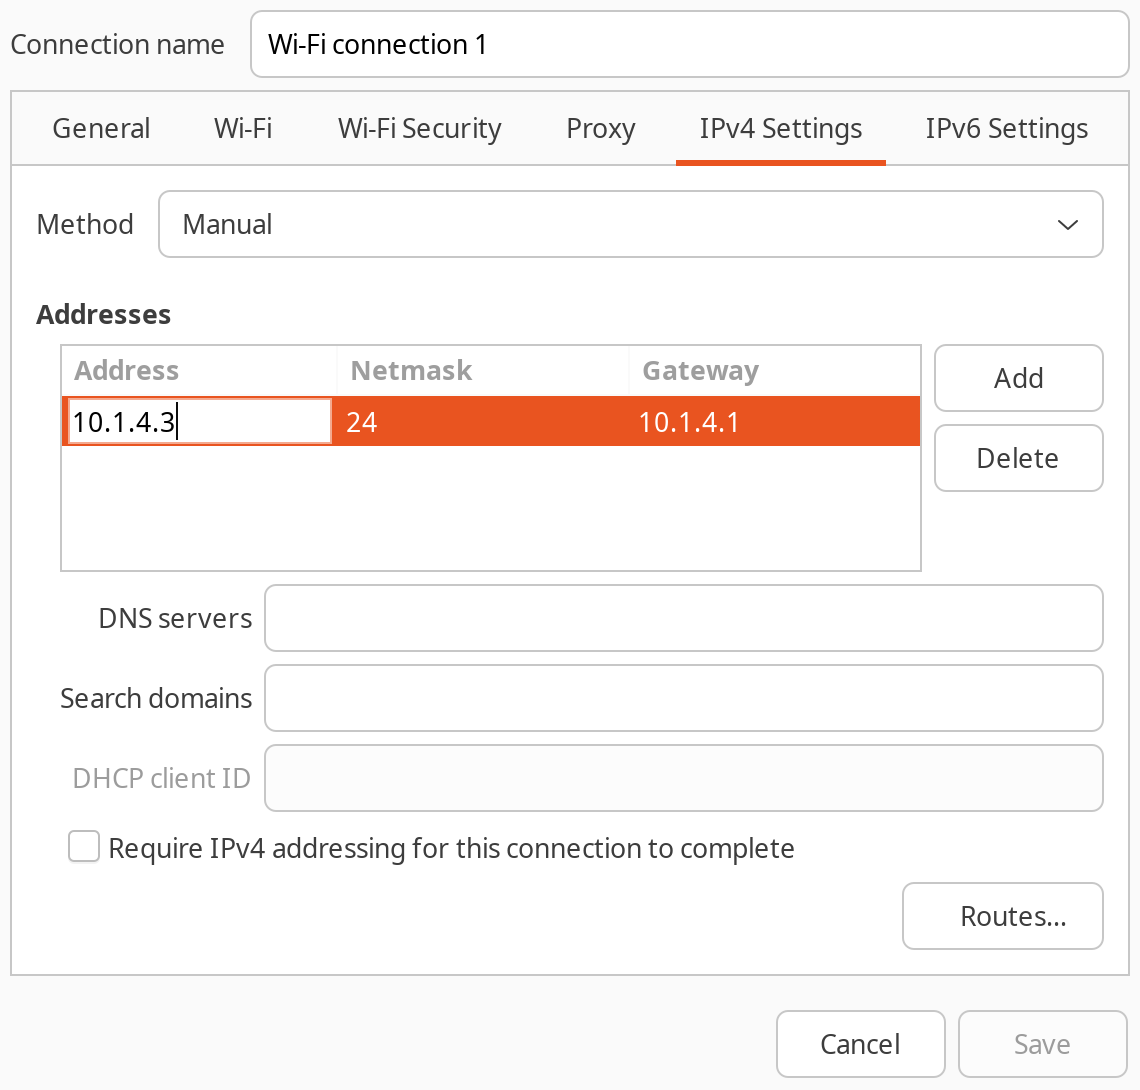
\includegraphics[width=0.5\textwidth]{../arp/ip-config-dialog}
\end{frame}

\begin{frame}{simple network config}
\begin{itemize}
    \item IP address: 10.0.2.45
    \item (sub)net mask: /25 (aka 255.255.255.128)
        \begin{itemize}
        \item varies which format is input
        \end{itemize}
    \item (default) gateway: 10.0.2.102
\end{itemize}
\begin{visibleenv}<2->
\begin{tikzpicture}
\matrix[tight matrix,
    column 1/.style={nodes={text width=4cm}},
    column 2/.style={nodes={text width=3cm}},
    column 3/.style={nodes={text width=2cm}},
] {
addresses \& next hop \& device \\
10.2.0.0/25 \& (direct) \& out \\
default \& 0.0.2.102 \& out \\
};
\end{tikzpicture}
\end{visibleenv}
\end{frame}

